\subsection{Sơ đồ hoạt động} \label{sec:activity_diagram}

Trong khi các bảng mô tả trường hợp sử dụng tập trung vào việc xác định các thành phần nghiệp vụ, sơ đồ hoạt động đóng vai trò minh họa các khía cạnh động của hệ thống. Các sơ đồ này chi tiết hóa luồng xử lý dữ liệu, các điểm quyết định và trình tự tương tác giữa các tác nhân với các thành phần hệ thống. Qua đó, nhóm có thể kiểm chứng tính logic của quy trình trước khi tiến hành cài đặt mã nguồn.

Tương tự như phần đặc tả chi tiết, trong phạm vi chương này nhóm trình bày các sơ đồ hoạt động cho những trường hợp sử dụng cốt lõi bao gồm các luồng tìm kiếm, đặt hàng, thanh toán và báo cáo quản trị thông qua các hình từ \ref{fig:act_find_product} đến \ref{fig:act_shopping_support}. Các sơ đồ hoạt động cho những nghiệp vụ hỗ trợ và quản lý khác được trình bày đầy đủ tại phần phụ lục \ref{sec:appx_activity_diagram} của đồ án.

\begin{figure}[H]
    \centering
    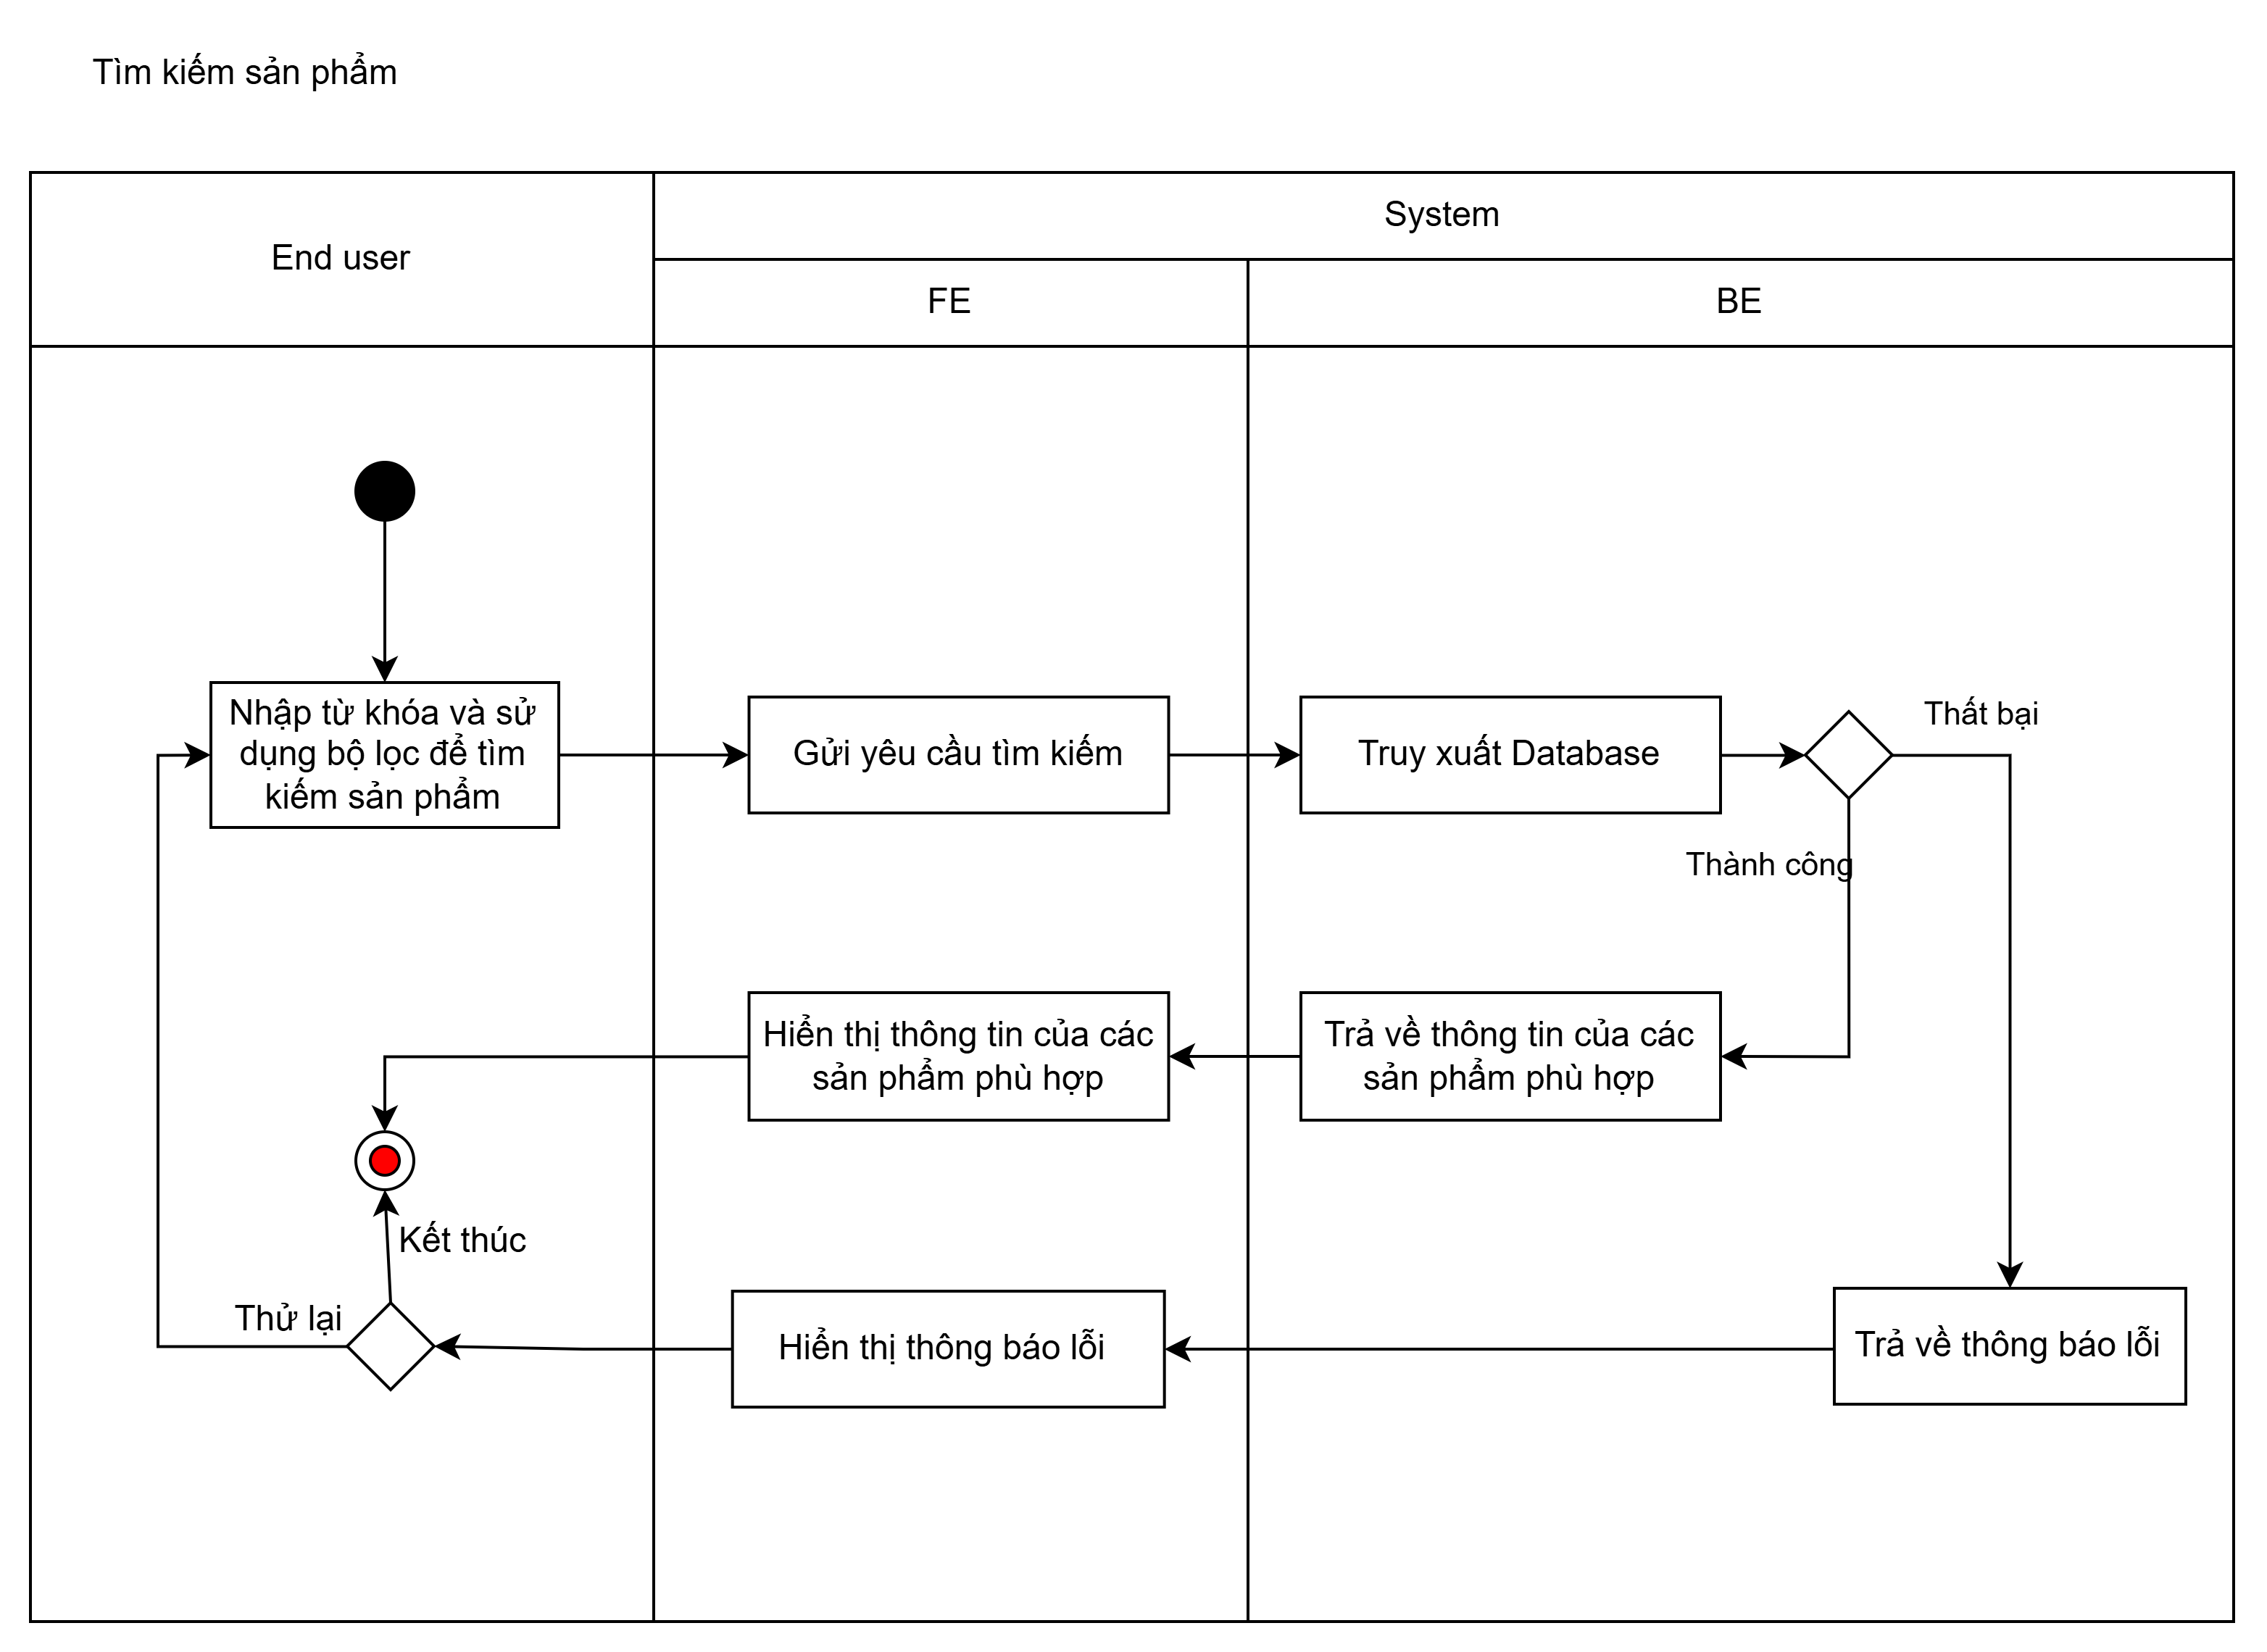
\includegraphics[width=0.8\linewidth]{images/chap3/activity_diagram/find_product.png}
   \vspace{0.5cm} \caption{Sơ đồ hoạt động Tìm kiếm sản phẩm}
    \label{fig:act_find_product}
\end{figure}
Hình \ref{fig:act_find_product} mô tả luồng người dùng nhập từ khóa hoặc chọn danh mục, hệ thống lọc dữ liệu và hiển thị danh sách sản phẩm phù hợp cùng chi tiết sản phẩm.

\begin{figure}[H]
    \centering
    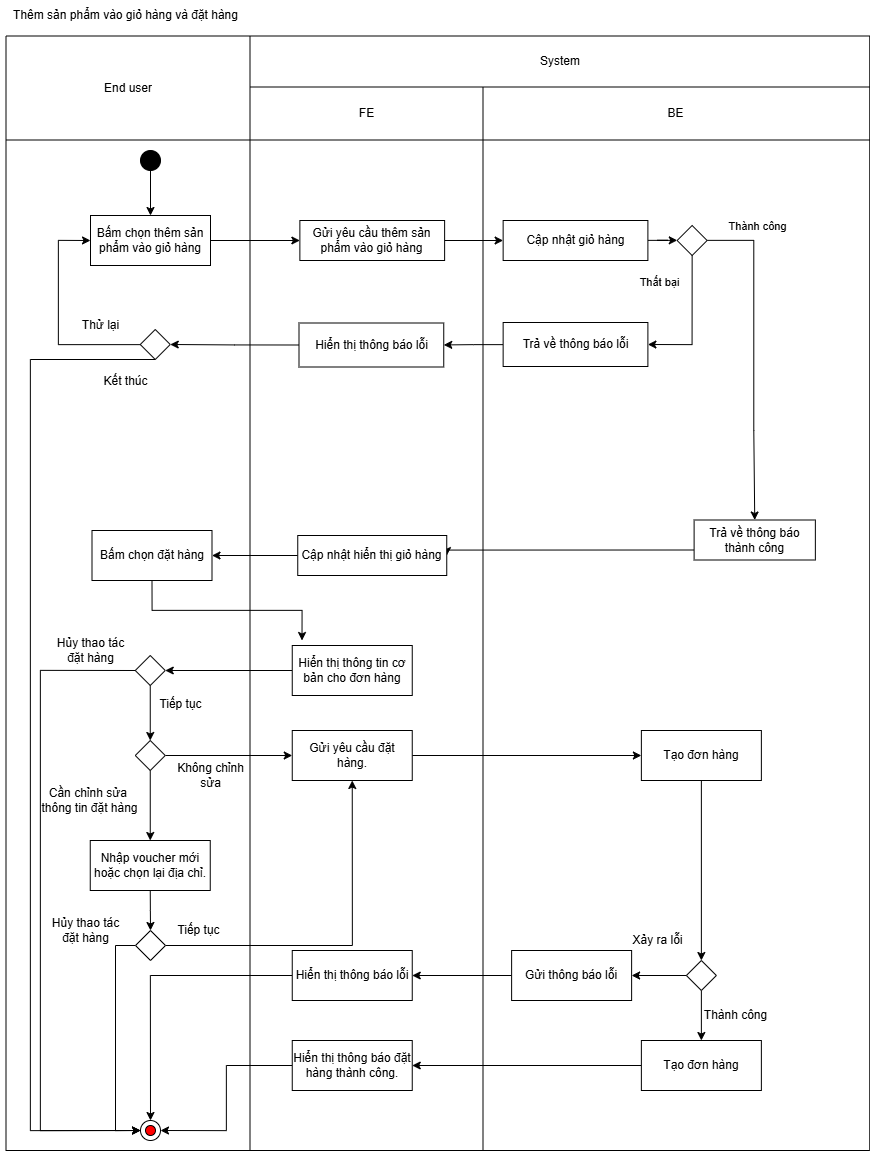
\includegraphics[width=0.8\linewidth]{images/chap3/activity_diagram/add_to_cart_and_checkout.png}
   \vspace{0.5cm} \caption{Sơ đồ hoạt động Thêm vào giỏ hàng và Đặt hàng}
    \label{fig:act_cart_checkout}
\end{figure}
Hình \ref{fig:act_cart_checkout} mô tả quy trình cốt lõi: Người dùng chọn sản phẩm, thêm vào giỏ, kiểm tra lại giỏ hàng, nhập thông tin giao hàng và xác nhận tạo đơn hàng.

\begin{figure}[H]
    \centering
    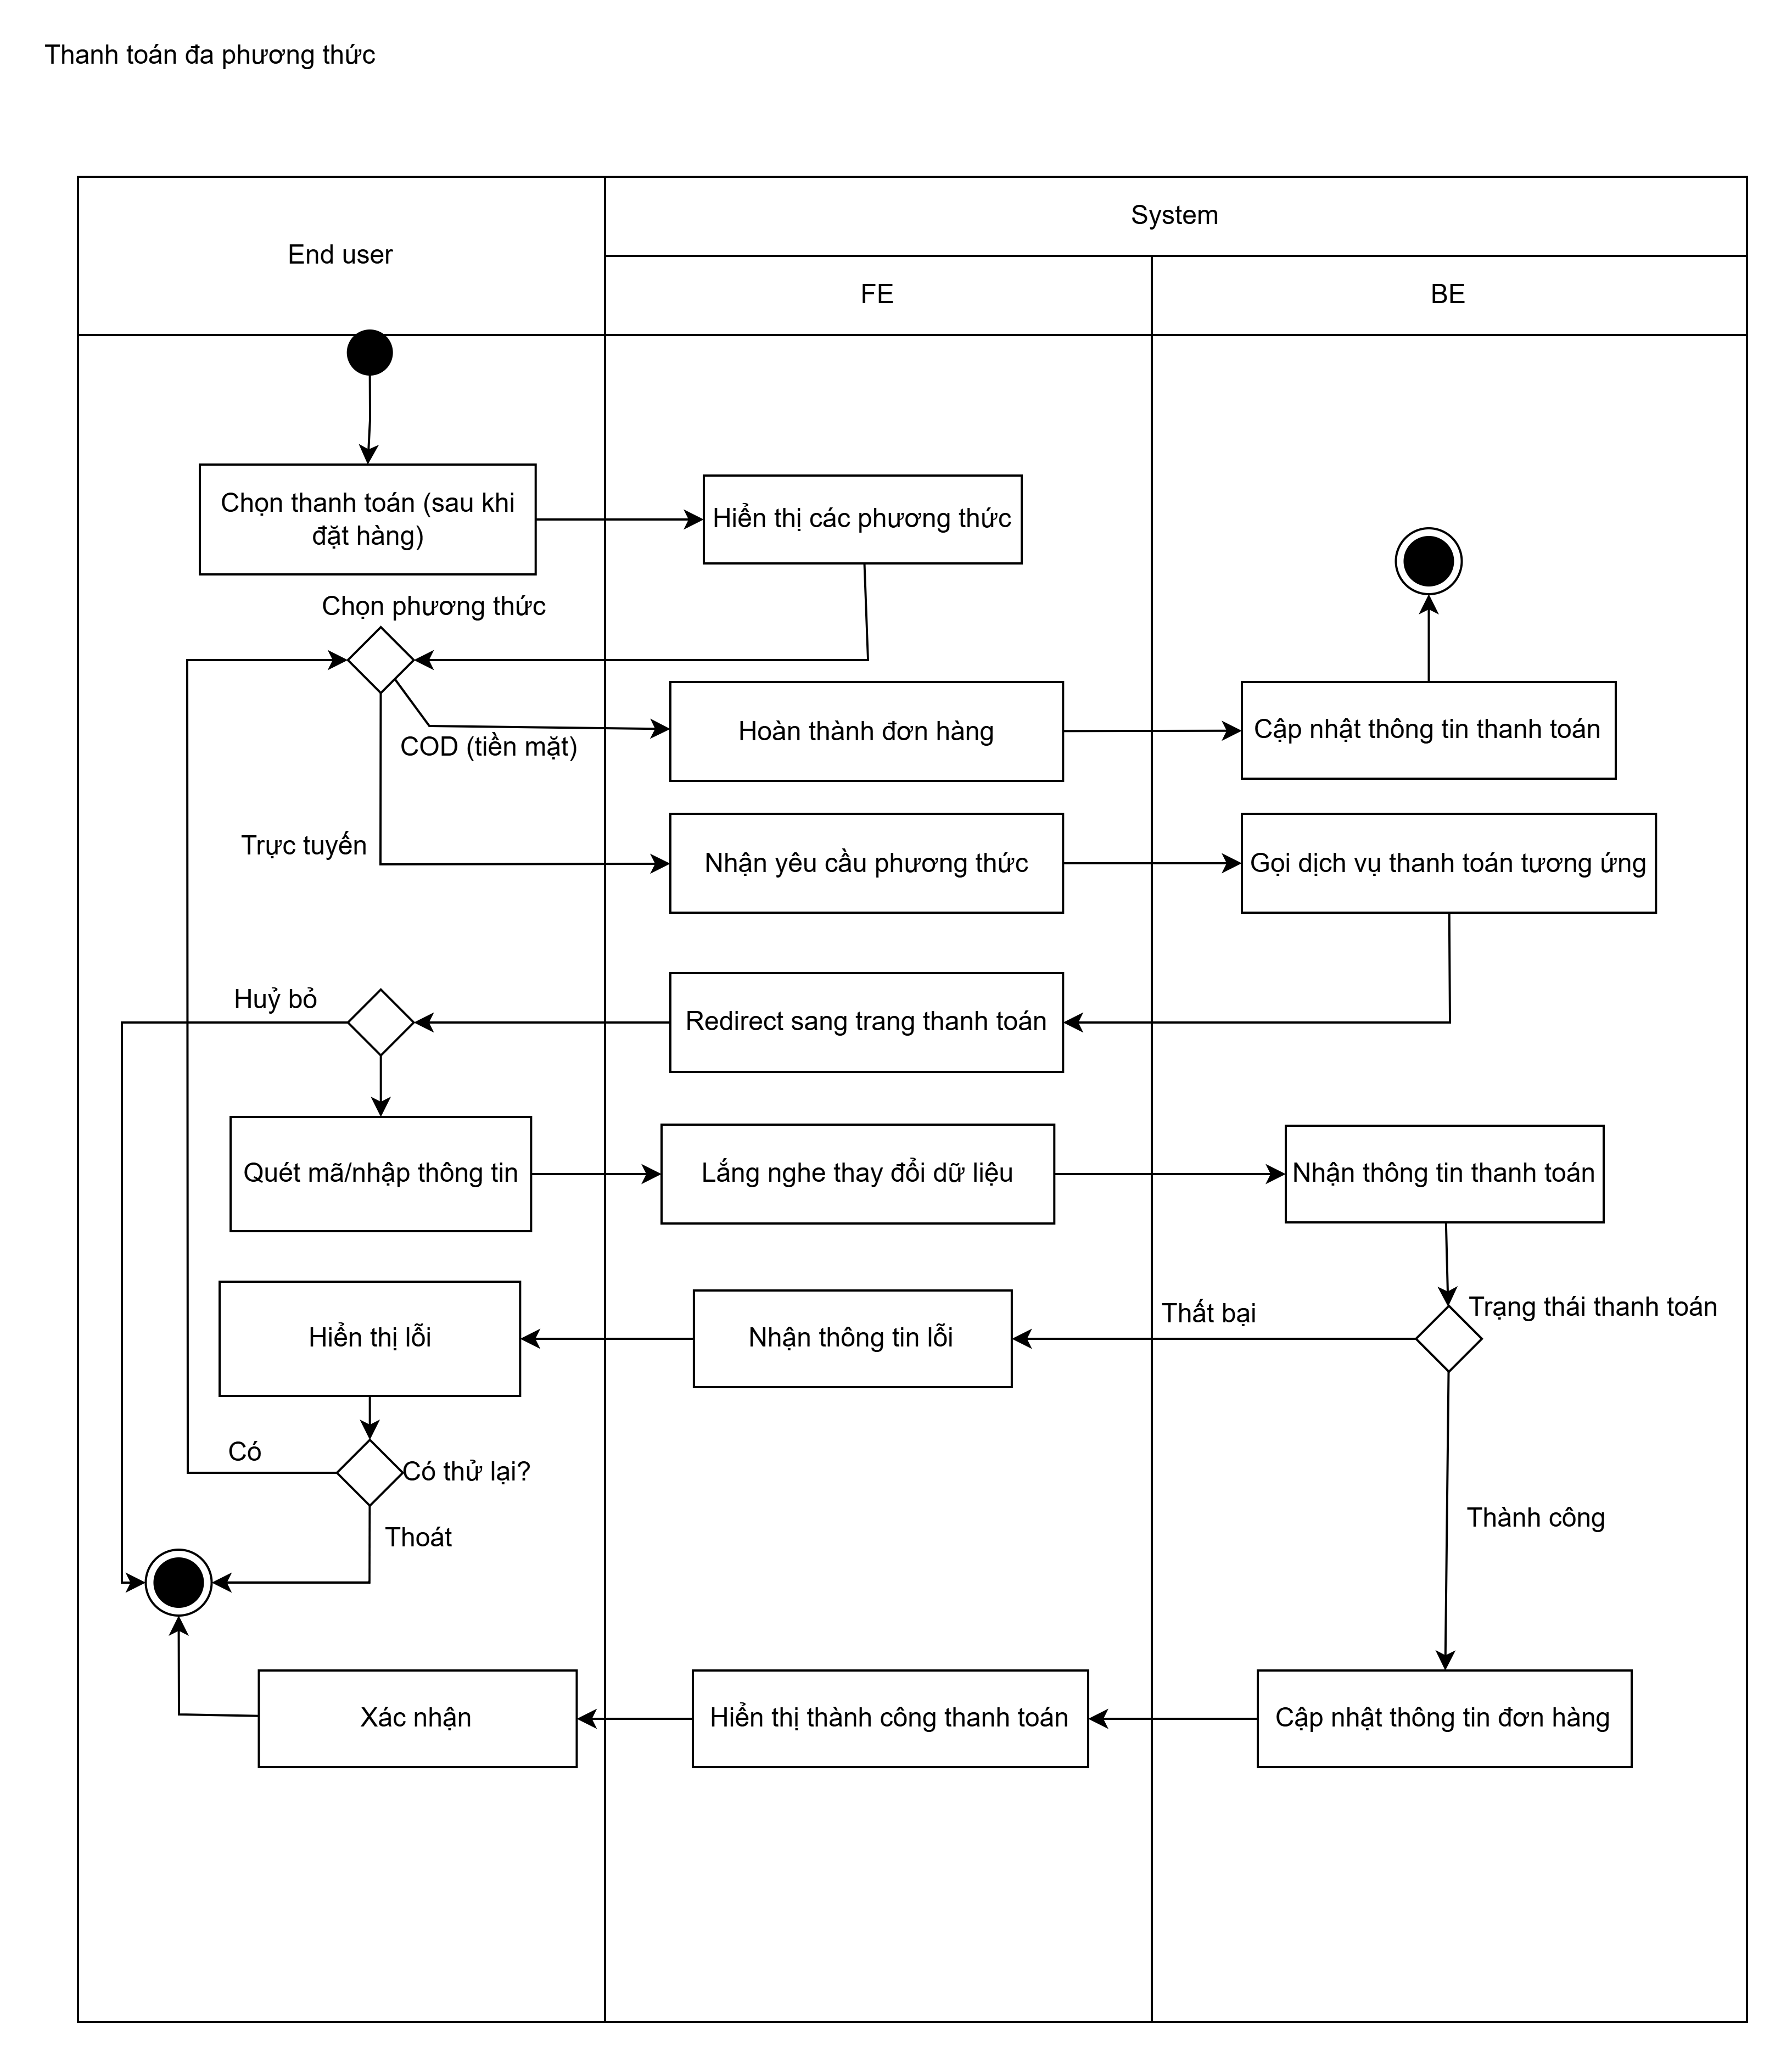
\includegraphics[width=0.8\linewidth]{images/chap3/activity_diagram/multiple_payment_method.png}
   \vspace{0.5cm} \caption{Sơ đồ hoạt động Lựa chọn phương thức thanh toán}
    \label{fig:act_payment}
\end{figure}
Hình \ref{fic:act_payment} chi tiết hóa bước thanh toán, cho phép người dùng chọn giữa các phương thức (COD, Ví điện tử, Chuyển khoản) và xử lý luồng giao dịch tương ứng.

\begin{figure}[H]
    \centering
    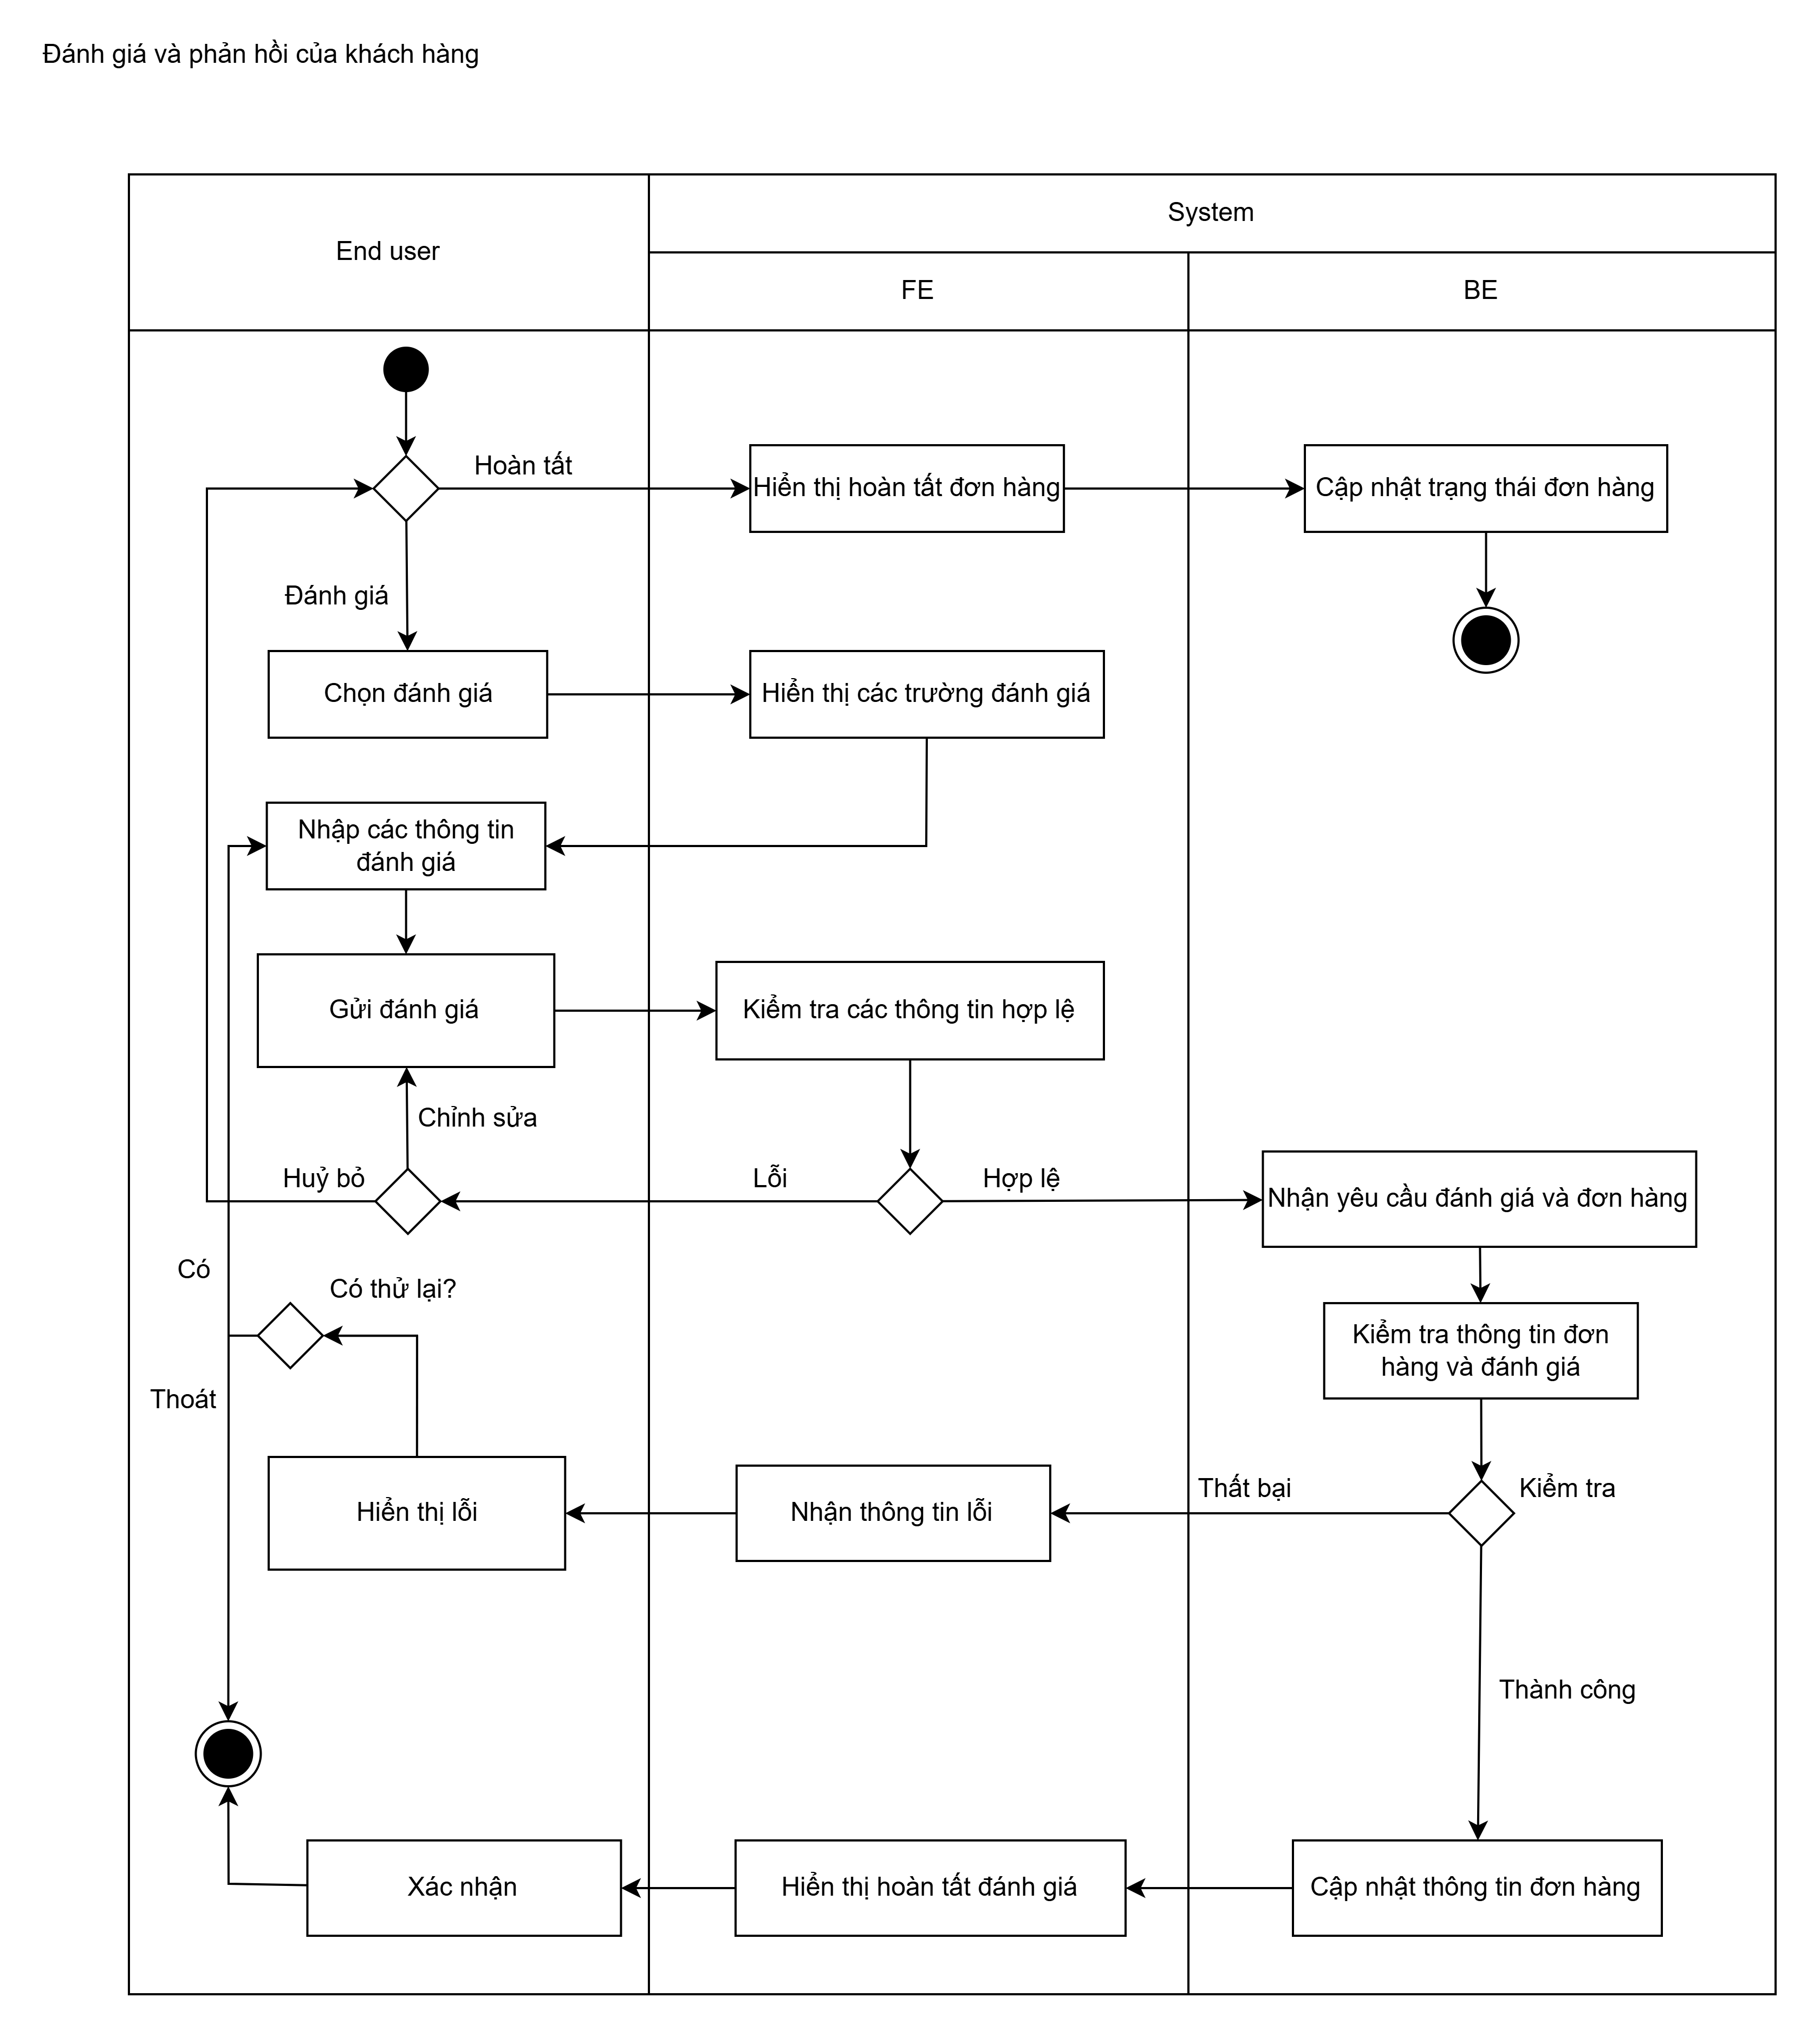
\includegraphics[width=0.7\linewidth]{images/chap3/activity_diagram/customer_feedback.png}
   \vspace{0.5cm} \caption{Sơ đồ hoạt động Phản hồi ý kiến khách hàng}
    \label{fig:act_feedback}
\end{figure}
Quy trình ghi nhận đánh giá, nhận xét của khách hàng về sản phẩm hoặc dịch vụ để cải thiện chất lượng hệ thống được biểu diễn ở hình \ref{fig:act_feedback}.

\begin{figure}[H]
    \centering
    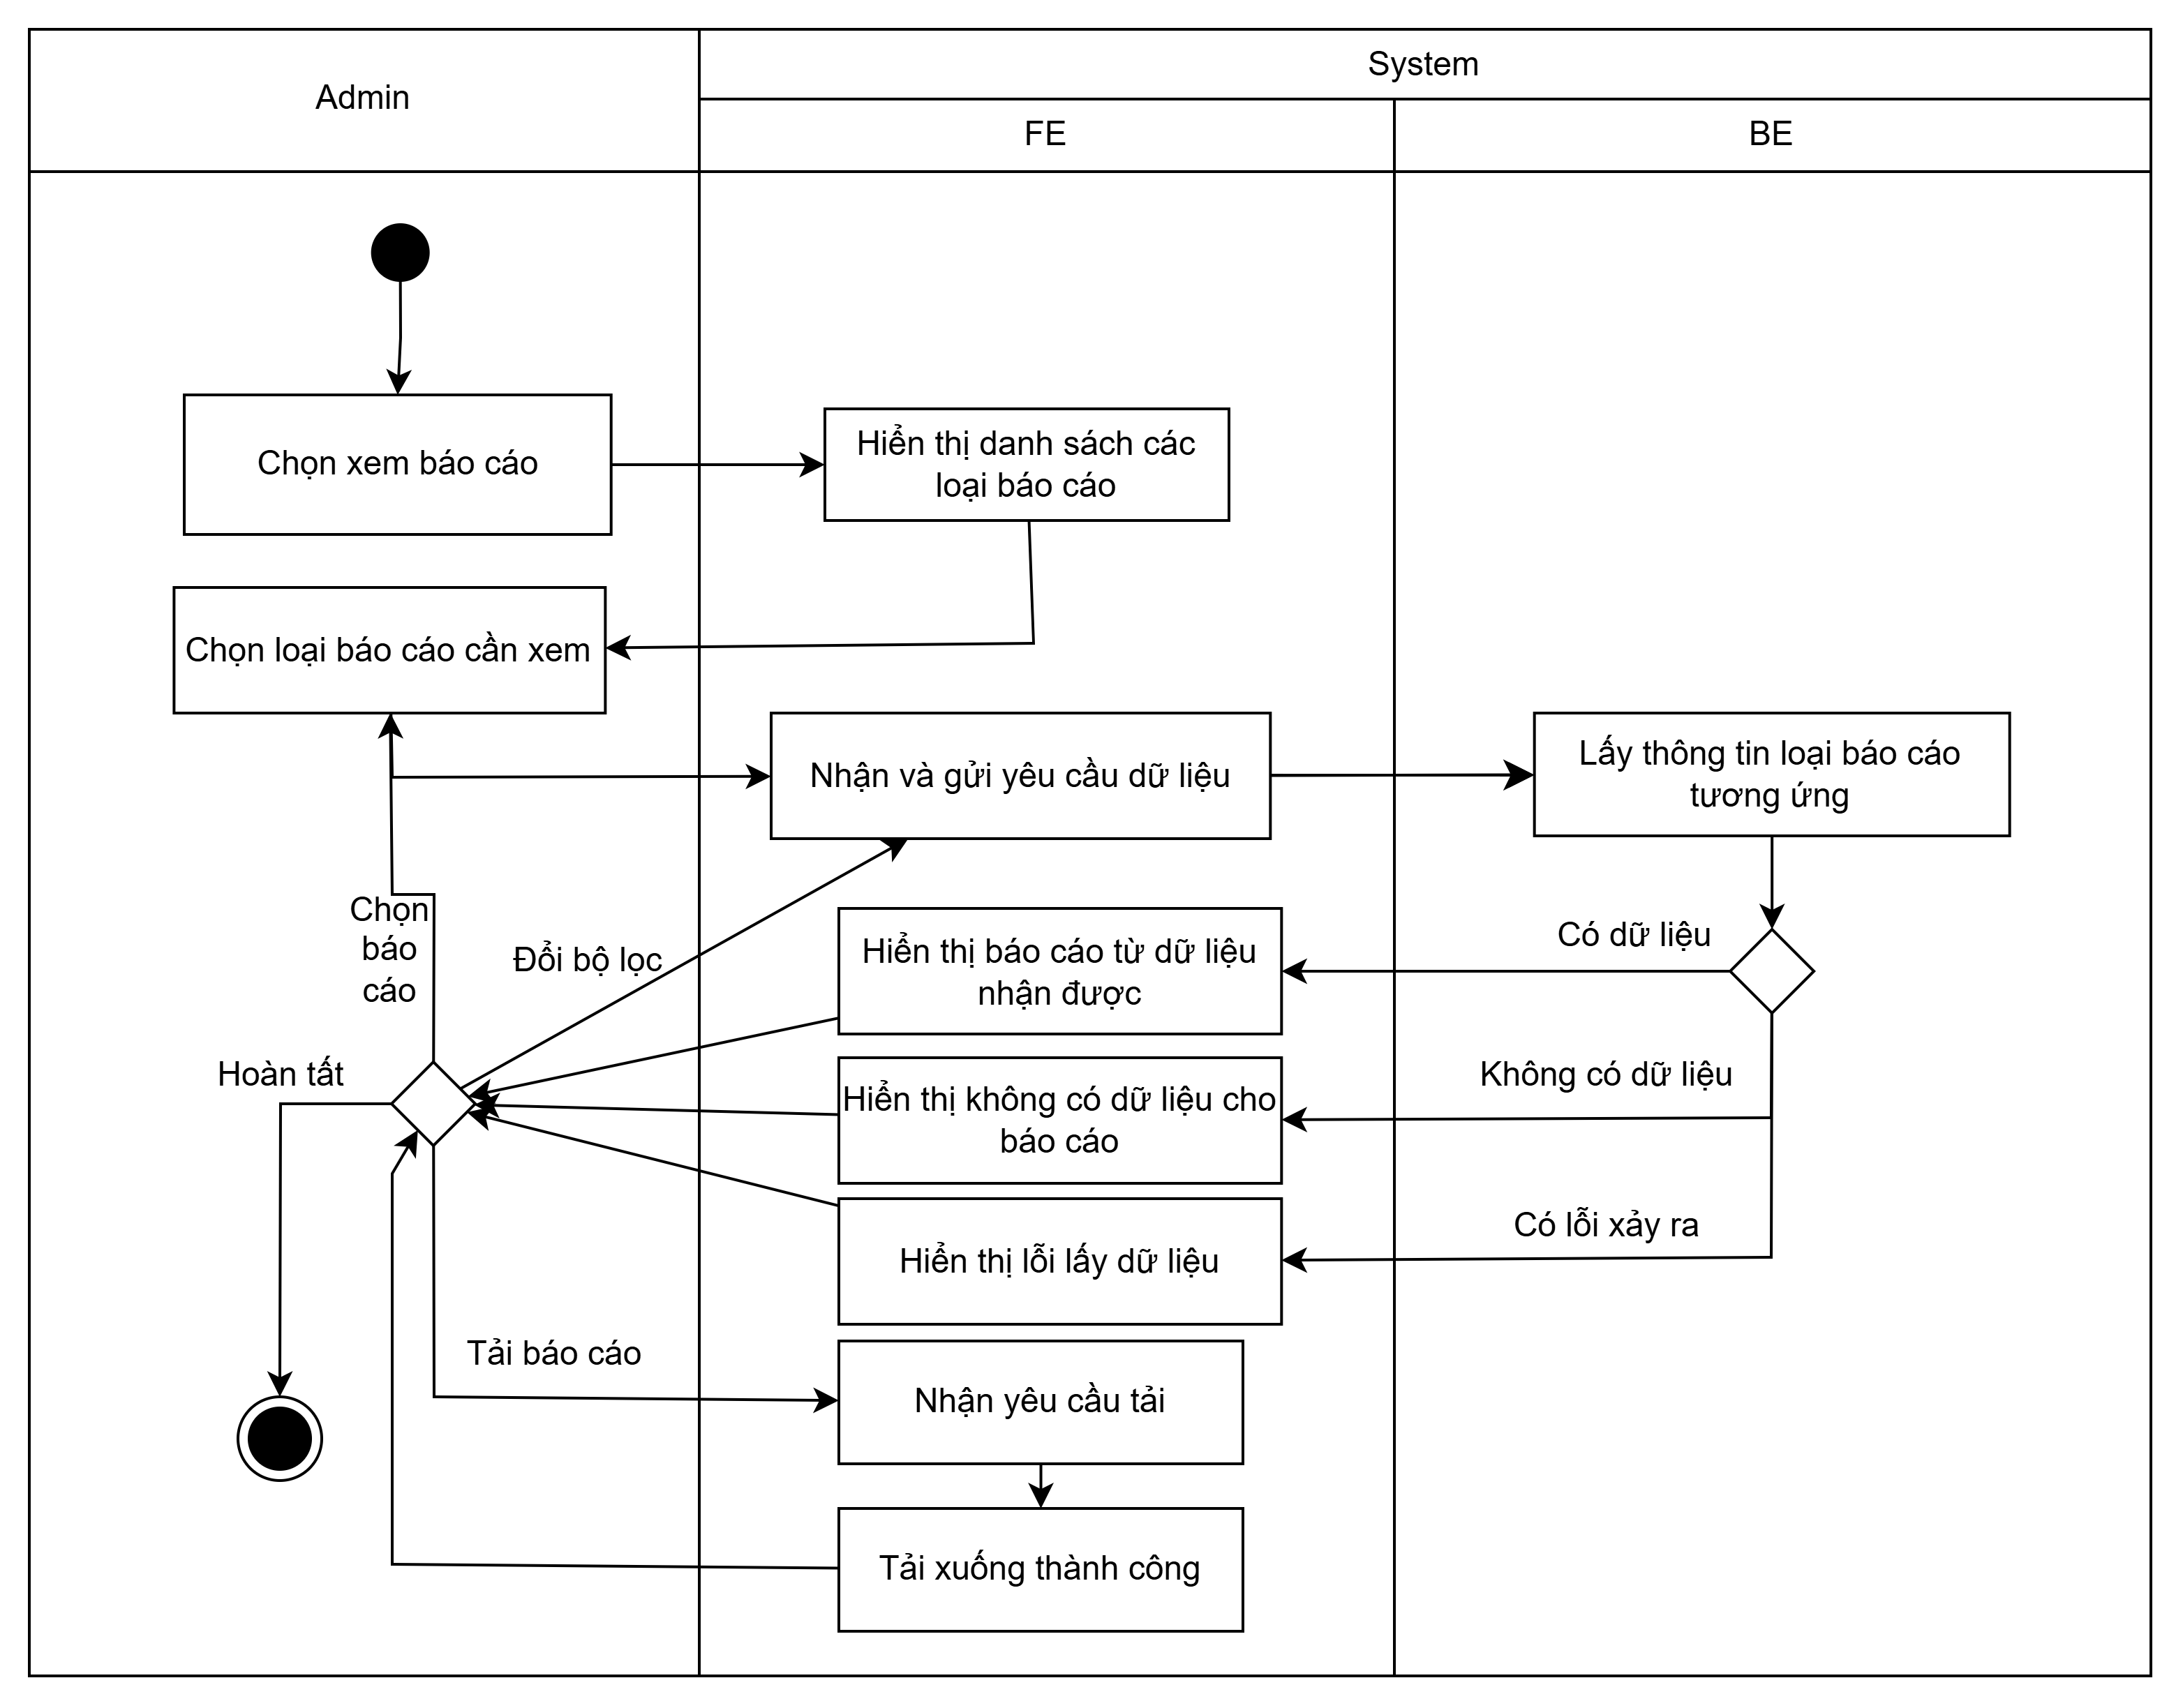
\includegraphics[width=0.8\linewidth]{images/chap3/activity_diagram/view_basic_report.png}
   \vspace{0.5cm} \caption{Sơ đồ hoạt động Xem báo cáo thống kê}
    \label{fig:act_report}
\end{figure}
Chức năng tổng hợp dữ liệu, hiển thị báo cáo doanh thu, số lượng đơn hàng và tồn kho cho người quản lý được biểu diễn qua hình \ref{fig:act_report}.

\begin{figure}[H]
    \centering
    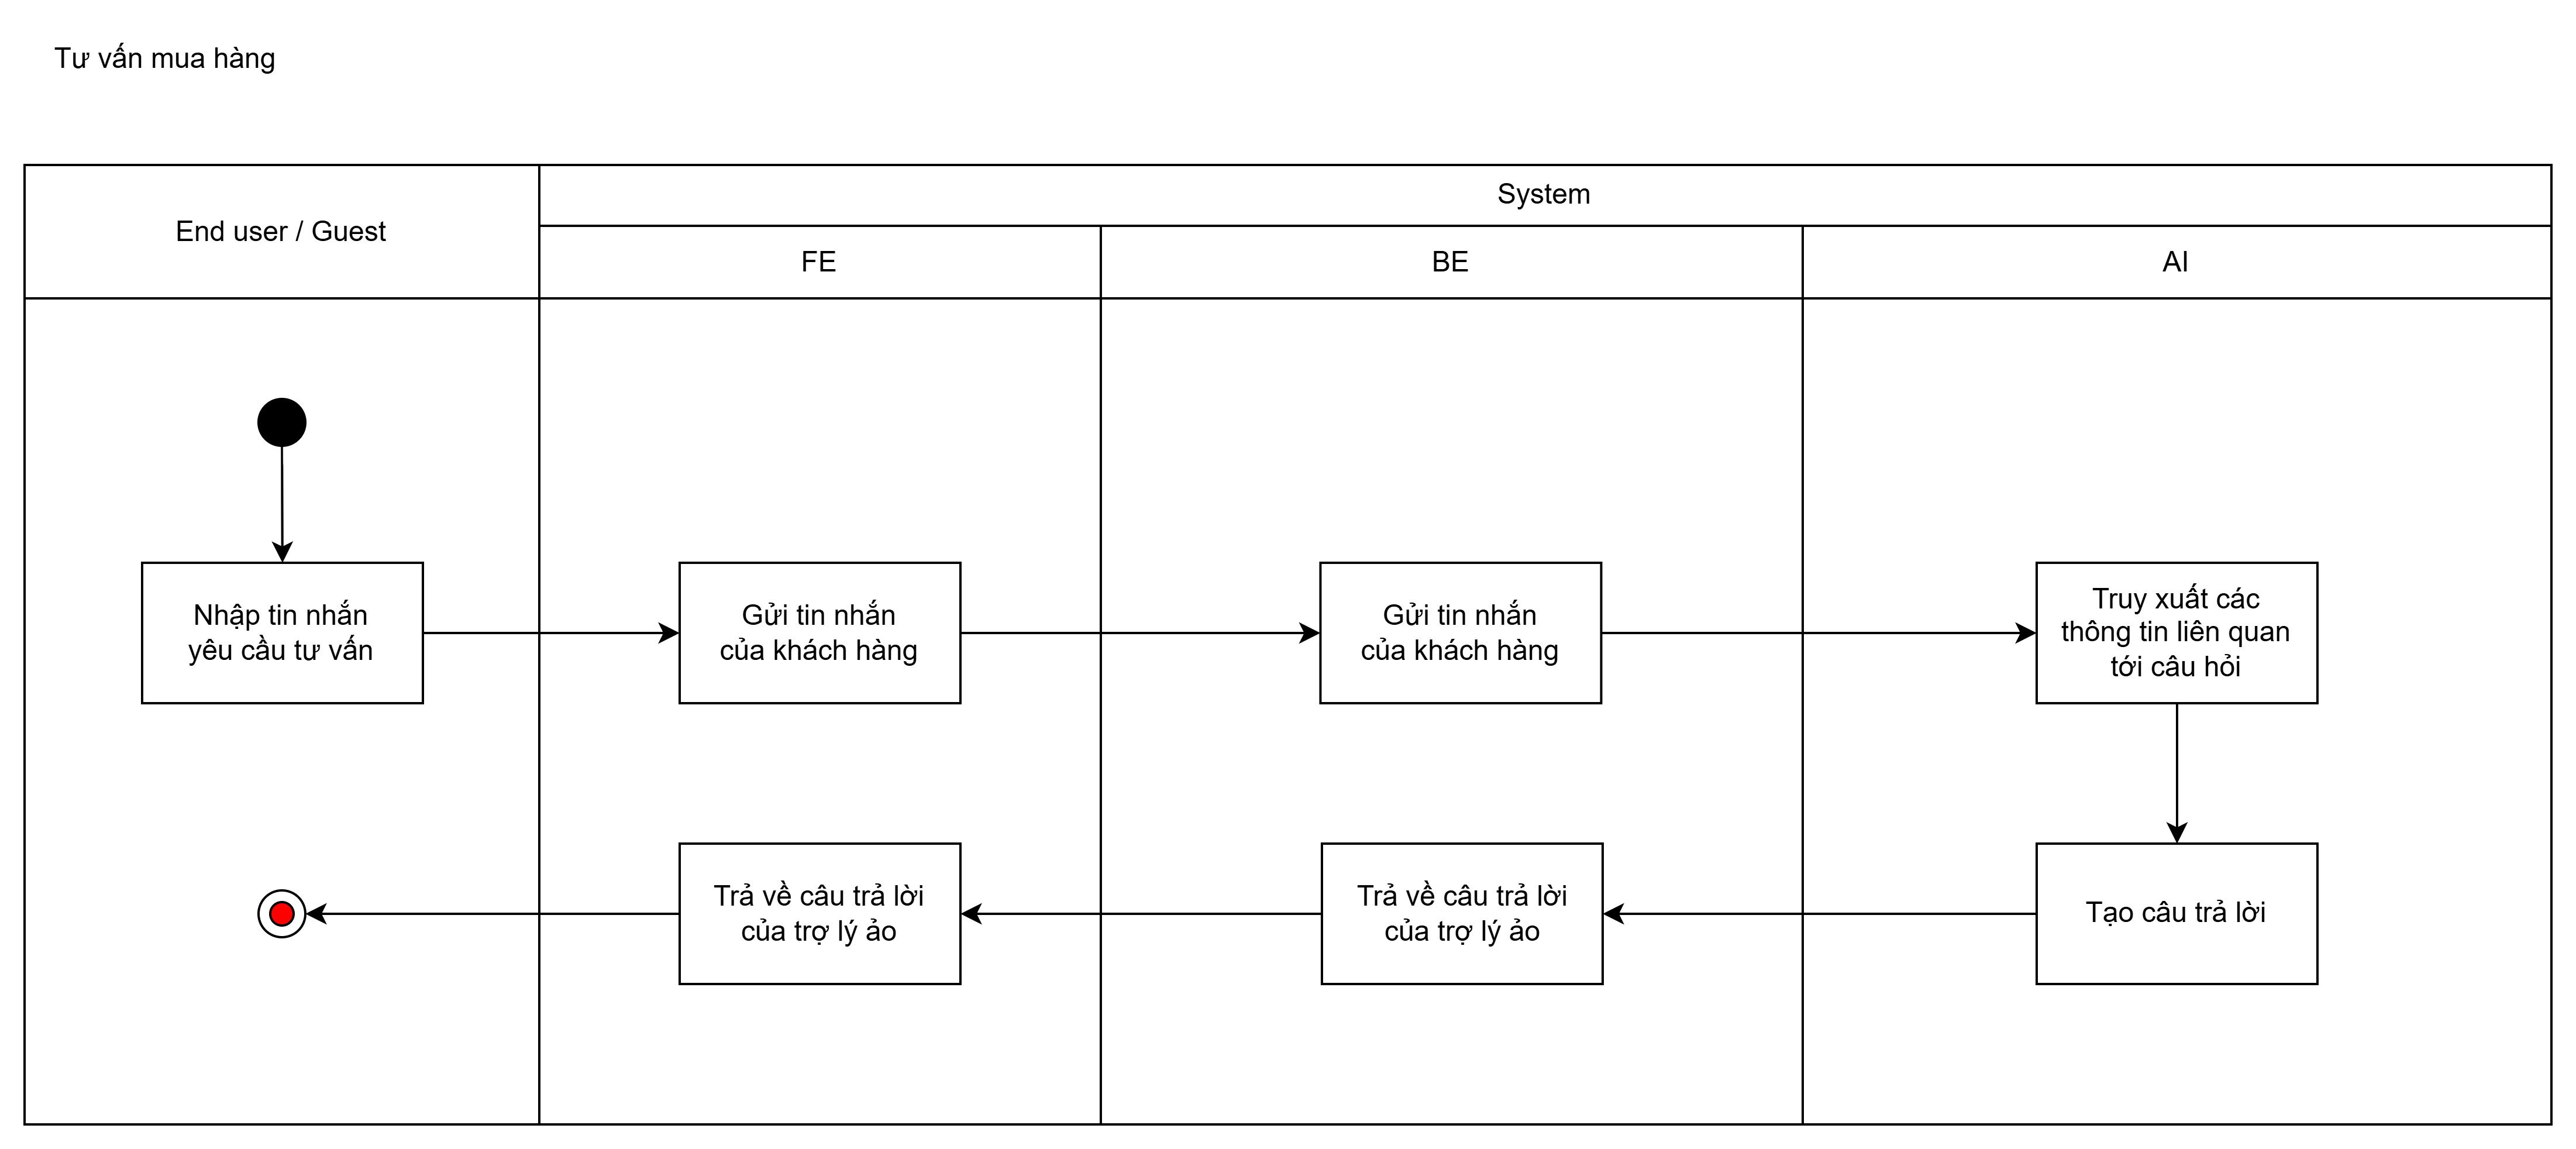
\includegraphics[width=0.8\linewidth]{images/chap3/activity_diagram/shopping_consulting.png}
   \vspace{0.5cm} \caption{Sơ đồ hoạt động Tư vấn mua sắm}
    \label{fig:act_consulting}
\end{figure}
Mô tả tương tác giữa khách hàng và nhân viên/chatbot để nhận tư vấn về thông tin sản phẩm trước khi quyết định mua.

\begin{figure}[H]
    \centering
    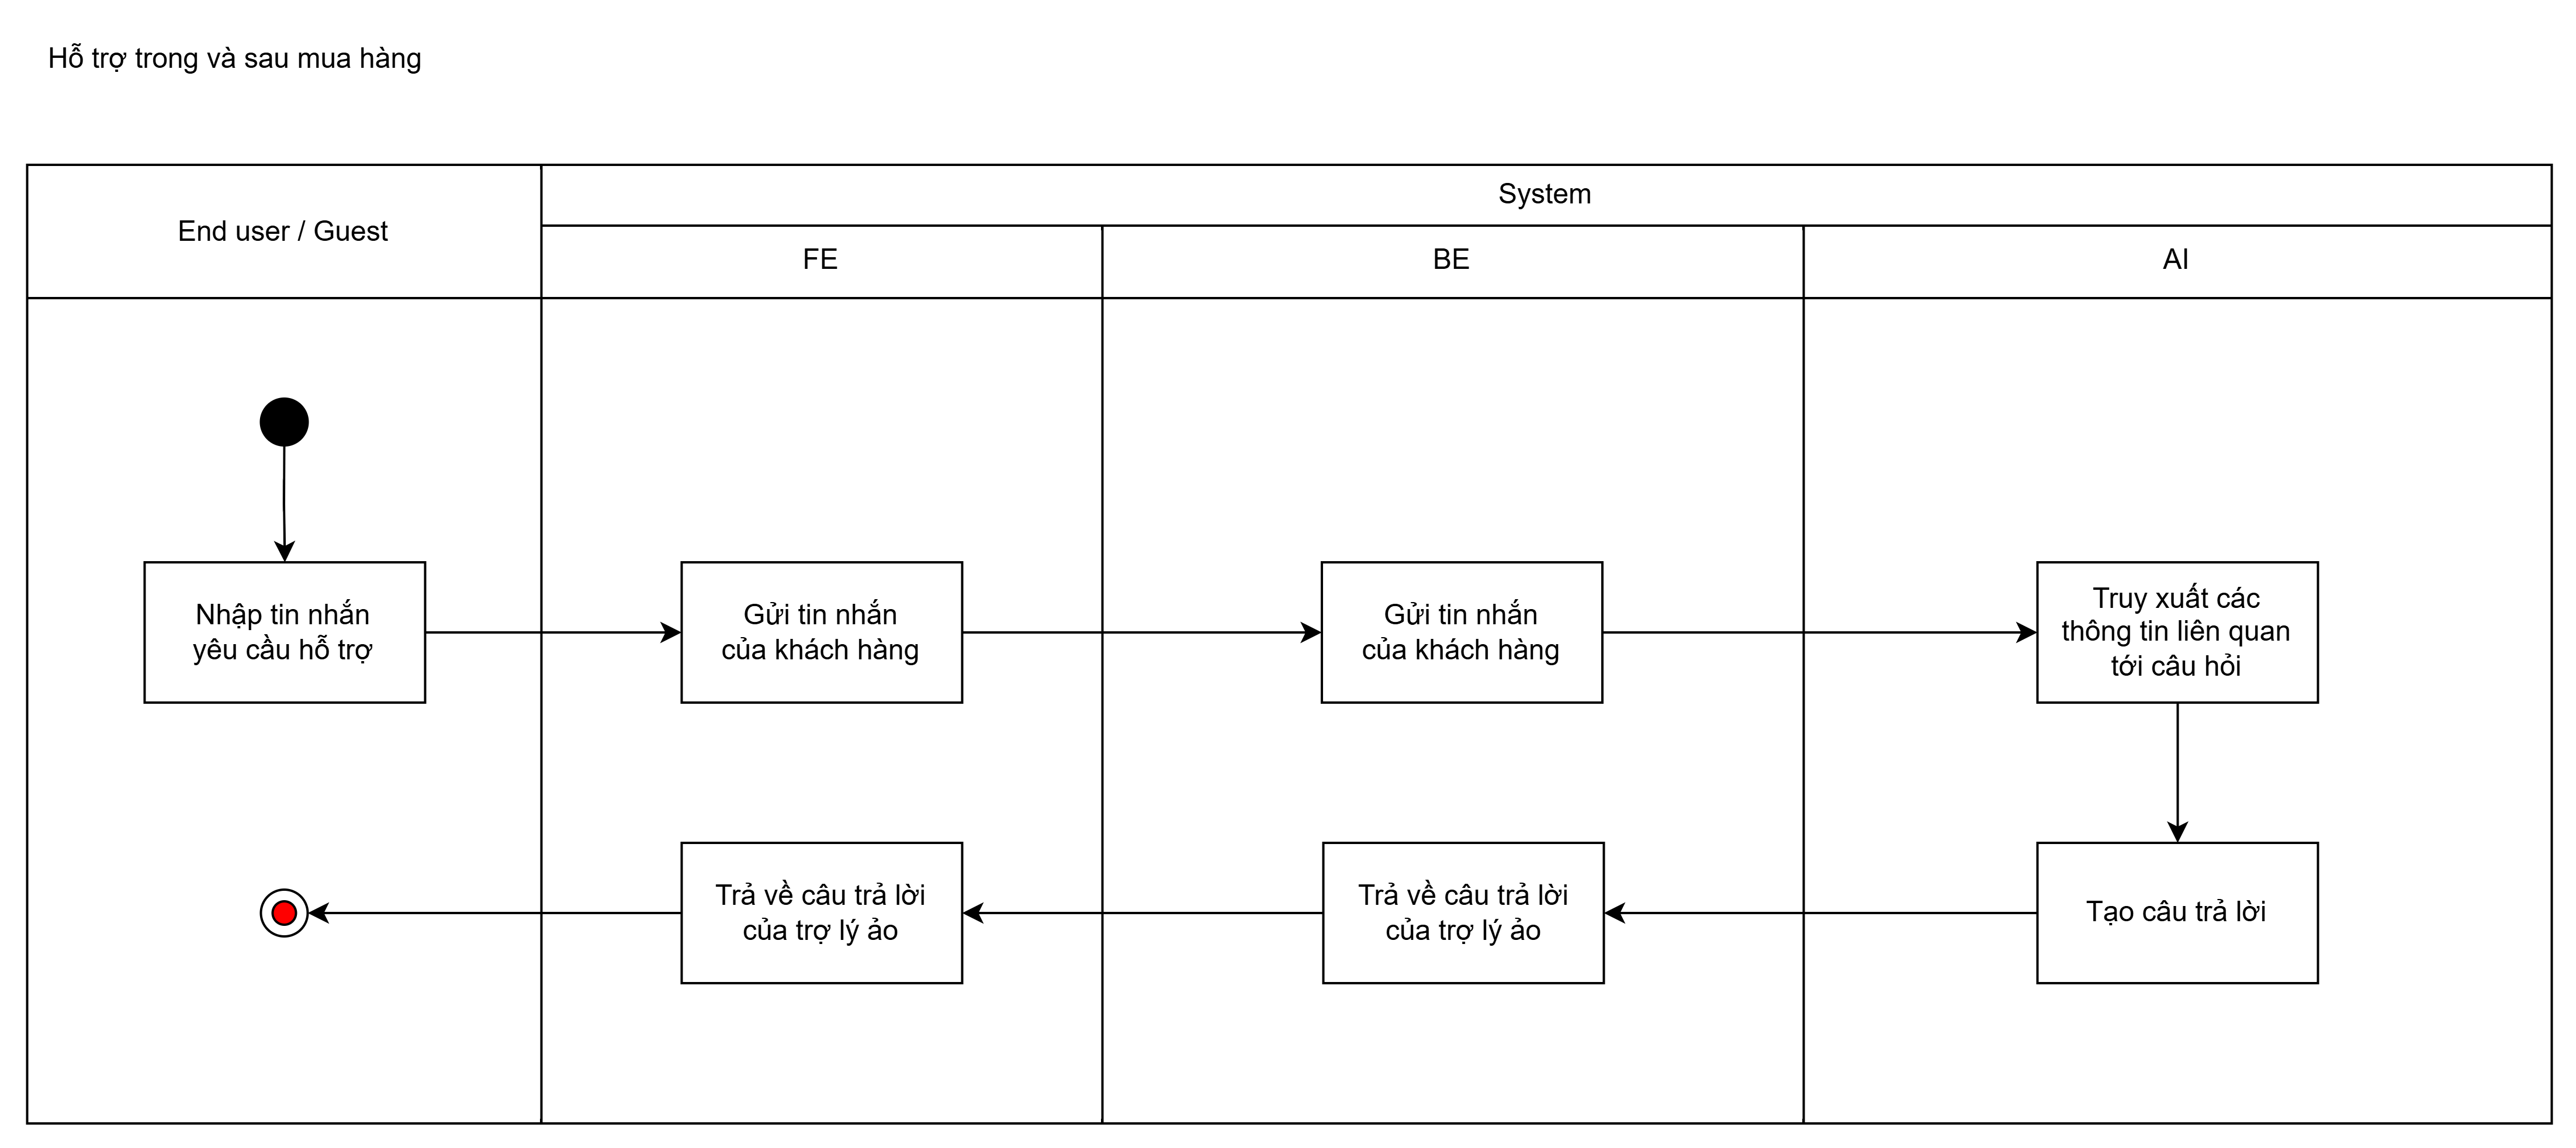
\includegraphics[width=0.8\linewidth]{images/chap3/activity_diagram/shopping_support.png}
   \vspace{0.5cm} \caption{Sơ đồ hoạt động Hỗ trợ sau bán hàng}
    \label{fig:act_shopping_support}
\end{figure}
Xử lý các yêu cầu khiếu nại, bảo hành hoặc các vấn đề phát sinh sau khi khách hàng đã nhận được sản phẩm.
